\begin{frame}{Context Window Problems}
  \begin{itemize}
    \item[\textcolor{red}{$\blacktriangleright$}] Current LLMs have a finite ``context window'':
      \begin{itemize}
        \item \textbf{GPT-3:} 2K tokens
        \item \textbf{GPT-4:} Up to 128K tokens
        \item \textbf{Claude 3.5:} Up to 200K tokens
      \end{itemize}
    \item[\textcolor{red}{$\blacktriangleright$}] \textbf{Problems:}
      \begin{itemize}
        \item Long documents get truncated
        \item Token limit affects reasoning
        \item Difficult to do document-level QA or summarization
      \end{itemize}
  \end{itemize}
\end{frame}

\begin{frame}{Context Window Problems}
  \begin{center}
    \textbf{Example of a Context Window}
    \vspace{1em}

    % A manual diagram in TikZ for a context window on a token sequence
    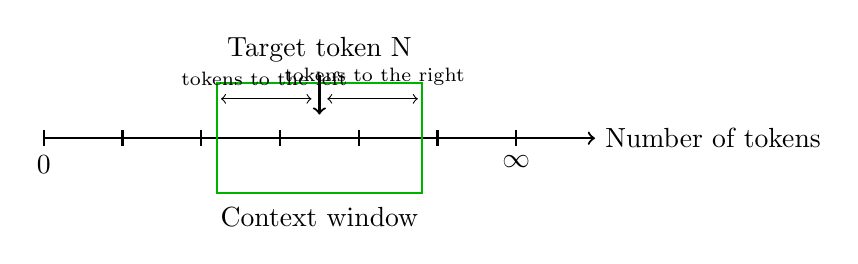
\begin{tikzpicture}[xscale=1.0, yscale=1]
      % Draw number line
      \draw[->, thick] (0,0) -- (7,0) node[right]{Number of tokens};
      % Tick marks and labels
      \foreach \x in {0,1,2,3,4,5,6}
        \draw[thick] (\x,0.1) -- (\x,-0.1);
      \node[below] at (0,-0.1) {0};
      \node[below] at (6,-0.1) {$\infty$};

      % Draw context window box
      \draw[thick, green!70!black] (2.2,0.7) -- (2.2,-0.7) -- (4.8,-0.7) -- (4.8,0.7) -- cycle;

      % Arrow to target token N
      \draw[->, thick] (3.5,0.8) -- (3.5,0.3);
      \node[above] at (3.5,0.85) {Target token N};

      % Arrows for left/right tokens
      \draw[<->] (2.25,0.5) -- (3.4,0.5);
      \node[above] at (2.8,0.55) {\scriptsize tokens to the left};
      \draw[<->] (3.6,0.5) -- (4.75,0.5);
      \node[above] at (4.2,0.55) {\scriptsize tokens to the right};

      % Label context window
      \node[below] at (3.5,-0.75) {Context window};
    \end{tikzpicture}
  \end{center}
\end{frame}

\begin{frame}{Context Window Problems}
  \begin{center}
    {\large \textbf{Why \textcolor{blue}{Bigger Context Windows} Aren't Always Better?}}
  \end{center}
  \vspace{1em}
  \begin{columns}[t,onlytextwidth]
    \begin{column}{0.24\textwidth}
      \fcolorbox{red}{white}{%
        \parbox{0.95\linewidth}{
          \centering
          \textbf{\textcolor{red}{1}}\\[0.3em]
          \textbf{Information Overload}\\[0.4em]
          {\scriptsize
          $\bullet$ Excess data can overwhelm the LLM.\\
          $\bullet$ Reduces focus and slows performance.
          }
        }
      }
    \end{column}
    \begin{column}{0.24\textwidth}
      \fcolorbox{orange}{white}{%
        \parbox{0.95\linewidth}{
          \centering
          \textbf{\textcolor{orange}{2}}\\[0.3em]
          \textbf{Getting Lost in Data}\\[0.4em]
          {\scriptsize
          $\bullet$ Large windows prioritize edges,\\ 
          $\bullet$ Missing key middle info.
          }
        }
      }
    \end{column}
    \begin{column}{0.24\textwidth}
      \fcolorbox{green}{white}{%
        \parbox{0.95\linewidth}{
          \centering
          \textbf{\textcolor{teal}{3}}\\[0.3em]
          \textbf{Poor Management}\\[0.4em]
          {\scriptsize
          $\bullet$ More data leads to noise,\\
          $\bullet$ Redundancy, and potential bias.
          }
        }
      }
    \end{column}
    \begin{column}{0.24\textwidth}
      \fcolorbox{black}{white}{%
        \parbox{0.95\linewidth}{
          \centering
          \textbf{4}\\[0.3em]
          \textbf{Long-Range Issues}\\[0.4em]
          {\scriptsize
          $\bullet$ Understanding relationships\\ 
          becomes harder with large context windows.
          }
        }
      }
    \end{column}
  \end{columns}
\end{frame}

\begin{frame}{Context Window Problems}
  \centering
  
\includegraphics[width=0.60\paperwidth,height=0.60\paperheight,keepaspectratio]{assets/Lecture-7_Large_Language_Models/pdf_page_065.png}
\end{frame}
